\documentclass{standalone}
\usepackage{tikz}
\usepackage{verbatim}
\begin{document}
\pagestyle{empty}
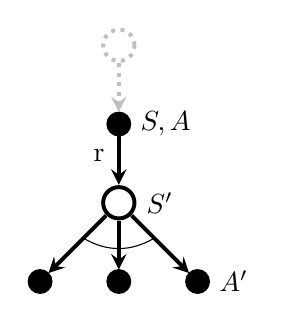
\begin{tikzpicture}

  % The graphic
  \node[draw,circle,scale=1.2, gray!50, dotted, fill=white, line width=0.5mm] (s_0) at (0,0) {};
  \node[draw,circle,scale=0.8, fill=black, line width=0.5mm, label=right:{$S,A$}] (a_0) at (0,-1) {};
  \node[draw,circle,scale=1.2, fill=white, line width=0.5mm, label=right:{$S'$}] (s_1) at (0,-2) {};
  \node[draw,circle,scale=0.8, fill=black, line width=0.5mm] (a_1) at (-1,-3) {};
  \node[draw,circle,scale=0.8, fill=black, line width=0.5mm] (a_2) at (0,-3) {};
  \node[draw,circle,scale=0.8, fill=black, line width=0.5mm, label=right:{$A'$}] (a_3) at (1,-3) {};
  \node (r) at (-0.25,-1.4) {r};
  
  
  \draw[-stealth, gray!50, dotted,line width=0.5mm] (s_0) -- (a_0);
  \draw[-stealth, line width=0.5mm] (a_0) -- (s_1);
  \draw[-stealth, line width=0.5mm] (s_1) -- (a_1);
  \draw[-stealth, line width=0.5mm] (s_1) -- (a_2);
  \draw[-stealth, line width=0.5mm] (s_1) -- (a_3);
  
  \path[-] (-.45,-2.45) edge[bend right=30] (.45, -2.45);
  
\end{tikzpicture}
\end{document}